\chapter{Formal analysis using Alloy}
It can be useful have a formal model for some of the main functionalities of Data4Help and AutomatedSOS. The following Alloy model explains in details the three core features of the system:

\begin{itemize}
\item The sending of an ambulance whenever the vital parameters of an individual, who has activated AutomatedSOS, crosses the given threshold. In particular, it is modelled the maximum reaction time.
\item The possibility that a third party can monitor the data of a specific individual. In particular, the model focuses on the fact that the individual must give permission to the third party in order to access his data.
\item The access to a collection of data by a third party. In particular, the systems must enforce a certain level of privacy.
\end{itemize}
For simplicity and without any loss of generality, all the entities that have a numeric value are represented with integer values in small intervals. Moreover, only upper thresholds for vital parameters are considered.

\section{Alloy model}

\definecolor{comment}{rgb}{0,0.6,0}
\definecolor{keyw}{rgb}{0,0,0.82}
\definecolor{num}{rgb}{0.5,0.5,0.5}
\definecolor{back}{rgb}{0.95,0.95,0.95}

\lstset{
backgroundcolor = \color{back},
morecomment=[l]{--},
morecomment=[s]{/*}{*/},
commentstyle = \color{comment},
morekeywords=[1]{open, sig, fact, one, Int, lone, set, some, extends, all, in, no, disj, and, or, implies, assert, check , run, pred, for},
keywordstyle = [1]{\color{keyw}},
basicstyle = \ttfamily,
frame=single,
breakatwhitespace = true,
breaklines = true,
rulecolor = \color{black},
tabsize = 3,
numbers = left,
numberstyle = \small\color{num},
literate=*
    {0}{{{\textcolor{red}0}}}1
    {1}{{{\textcolor{red}1}}}1
    {2}{{{\textcolor{red}2}}}1
    {3}{{{\textcolor{red}3}}}1
    {4}{{{\textcolor{red}4}}}1
    {5}{{{\textcolor{red}5}}}1
    {6}{{{\textcolor{red}6}}}1
    {7}{{{\textcolor{red}7}}}1
    {8}{{{\textcolor{red}8}}}1
    {9}{{{\textcolor{red}9}}}1,
    escapeinside={!}{!},
}

\begin{lstlisting}
open util/integer
open util/boolean

sig Location {
	coordX: one Int,
	coordY: one Int
}
{coordX >= -3 and coordX <= 3 and coordY >= -6 and coordY <= 6}

sig Time {
	time: one Int
}
{time >= 0 and time <= 6}

sig Individual {
	hasSOS: one Bool,
	data: lone EHealthData,
	location: lone Location,
	illness: lone Illness
}

sig EHealthData {
	heartRate: lone Int,
	bloodPressure: lone Int,
	steps: lone Int,
	sleepTime: lone Int	
}
{heartRate >= 0 and heartRate <= 6 and bloodPressure >= 0 and bloodPressure <= 6 and steps >= 0 and steps <= 6 and sleepTime >= 0 and sleepTime <= 6}

sig Illness {
	startTime: one Time
}

sig Ambulance {
	startTime: one Time,
	rescuee: one Individual,
	location: one Location
}

sig EHealthDataGroup {
	data: some EHealthData 
}

sig ThirdParty {
	request: set Request,
	monitor: set Individual,
	groupData: set EHealthDataGroup
}

abstract sig Request {
	approved: one Bool
}

sig GroupRequest extends Request {
	groupData: one EHealthDataGroup
}

sig SpecificRequest extends Request {
	individual: one Individual
}



/*
	Ambulance sending
*/

-- Every EHealthData belongs to a single Individual
fact DataBelongsToSingleIndividual {
	(all d: EHealthData | one i: Individual | i.data = d) 
}

-- There is a Ilness iff threshold have been crossed
fact IllnessIndividual{
	(all i: Individual | i.hasSOS = True and (i.data.heartRate >= 5 or i.data.bloodPressure >= 5) implies one il: Illness | il = i.illness) and	(all il: Illness | one i: Individual | il = i.illness and i.hasSOS = True and (i.data.heartRate >= 5 or i.data.bloodPressure >= 5))
}

-- Prevent two individual with same Illness
fact IllnessSigleIndividual {
	all il: Illness | no disj !i1!, !i2!: Individual | il = !i1!.illness and il = i!2!.illness
}

-- An ambulance is sent for a good reason with a reaction time of less than 2
fact AmbulanceIndividual {
	all a: Ambulance | a.rescuee.location = a.location and #a.rescuee.illness = 1 and a.startTime.time >= a.rescuee.illness.startTime.time and minus[a.startTime.time, a.rescuee.illness.startTime.time] <= 2
}

-- If an Individual is having an illness and he hade activate AutomatedSOS then an Ambulance is directed to his location.
-- Constraint also that only one ambulance has been sent
fact IndividualAmbulance {
	all i: Individual | #i.illness = 1 implies one a: Ambulance | a.rescuee = i
}



/*
	Requests
*/

-- Every request has been sent by a single ThirdParty
fact RequestThirdParty {
	(all r: Request | one t: ThirdParty | r in t.request ) 
}


/* Specific Requests */

-- A third party monitor only individuals who has accepted to be monitored
fact IndividualMonitored {
	all t: ThirdParty | all i: Individual | i in t.monitor implies 		one r: SpecificRequest | i = r.individual and r.approved = True and r in t.request
}

-- If a SpecificRequest is approved, a ThirdParty is monitoring the specific Individual
fact SpecificRequestApproved {
	all t: ThirdParty | all r: SpecificRequest | r in t.request and r.approved = True implies r.individual in t.monitor
}

-- No multiple SpecificRequest for the same Individual from the same ThirdParty
fact NoMultipleSpecificRequest {
	all t: ThirdParty | no disj r!1!, r!2!: SpecificRequest | r!1! in t.request and r!2! in t.request and r!1!.individual = r!2!.individual
}


/* Group Requests */

-- If TrackMe can properly anonymized those a EHealthDataGroup, a GroupRequest to this group is automatically accepted
fact GroupDataPrivacy {
	all r: GroupRequest | #r.groupData.data > 3 implies r.approved = True else r.approved = False
}

-- If a ThirdParty have access to a group of data then there is an approved request for them
fact GroupDataRequest {
	all t: ThirdParty | all g: EHealthDataGroup | g in t.groupData implies (one r: GroupRequest | r in t.request and r.groupData = g and r.approved = True)
}

-- If a GroupRequest is accepted, then the ThirdParty have access to EHealthDataGroup
fact {
	all t: ThirdParty | all r: GroupRequest | r in t.request and r.approved = True implies r.groupData in t.groupData
}

-- No multiple GroupRequest for the same group from the same ThirdParty
fact {
	all t: ThirdParty | no disj r!1!, r!2!: GroupRequest | r!1! in t.request and r!2! in t.request and r!1!.groupData = r!2!.groupData
}




pred ambulanceWorld {
	some i: Individual | #i.illness > 0 and some a: Ambulance | a.rescuee = i and a.startTime.time > i.illness.startTime.time
}

run ambulanceWorld for 4 but 1 Ambulance, 1 Individual, 1 Illness, 5 Int


pred groupRequestWorld {
	some r!1!, r!2!: GroupRequest | r!1!.approved = True and r!2!.approved = False
}

run groupRequestWorld for 6 but 2 Request, 1 ThirdParty, 5 Int


pred specificRequestWorld {
	some r!1!, r!2!: SpecificRequest | r!1!.approved = True and r!2!.approved = False
}

run specificRequestWorld for 5 but 2 Request, 2 Individual, 1 ThirdParty, 2 EHealthData, 0 EHealthDataGroup, 5 Int

assert privacyMaintained {
	no d: EHealthDataGroup | some t: ThirdParty | d in t.groupData and #d.data <= 3
}

check privacyMaintained for 15

assert monitorAccepted {
	no i: Individual | some t: ThirdParty | i in t.monitor and no r: SpecificRequest | r.approved = True and r in t.request
}

check monitorAccepted for 15

assert ambulanceCalling {
	no i: Individual | #i.illness > 0 and no a: Ambulance | a.rescuee = i and a.location = i.location
}

check ambulanceCalling for 15

assert ambulanceReactionTime {
	no i: Individual | #i.illness > 0 and some a: Ambulance | a.rescuee = i and a.location = i.location and minus[a.startTime.time, a.rescuee.illness.startTime.time] > 2
}

check ambulanceReactionTime for 15
\end{lstlisting}




\section{Worlds generated}

\subsection{Ambulance}
In Figure \ref{f:ambWorld}, it is shown that an ambulance is sent to the location of an Individual that he doesn't feel good.
Note that it can be there a (bounded) delay between the moment in which the vital parameters cross the thresholds (start of the Illness) and the time in which the ambulance is alerted.
\begin{lstlisting}[numbers=none]
run ambulanceWorld for 4 but 1 Ambulance, 1 Individual, 1 Illness, 5 Int
\end{lstlisting}

\begin{figure}[!ht]
\centering
\fbox{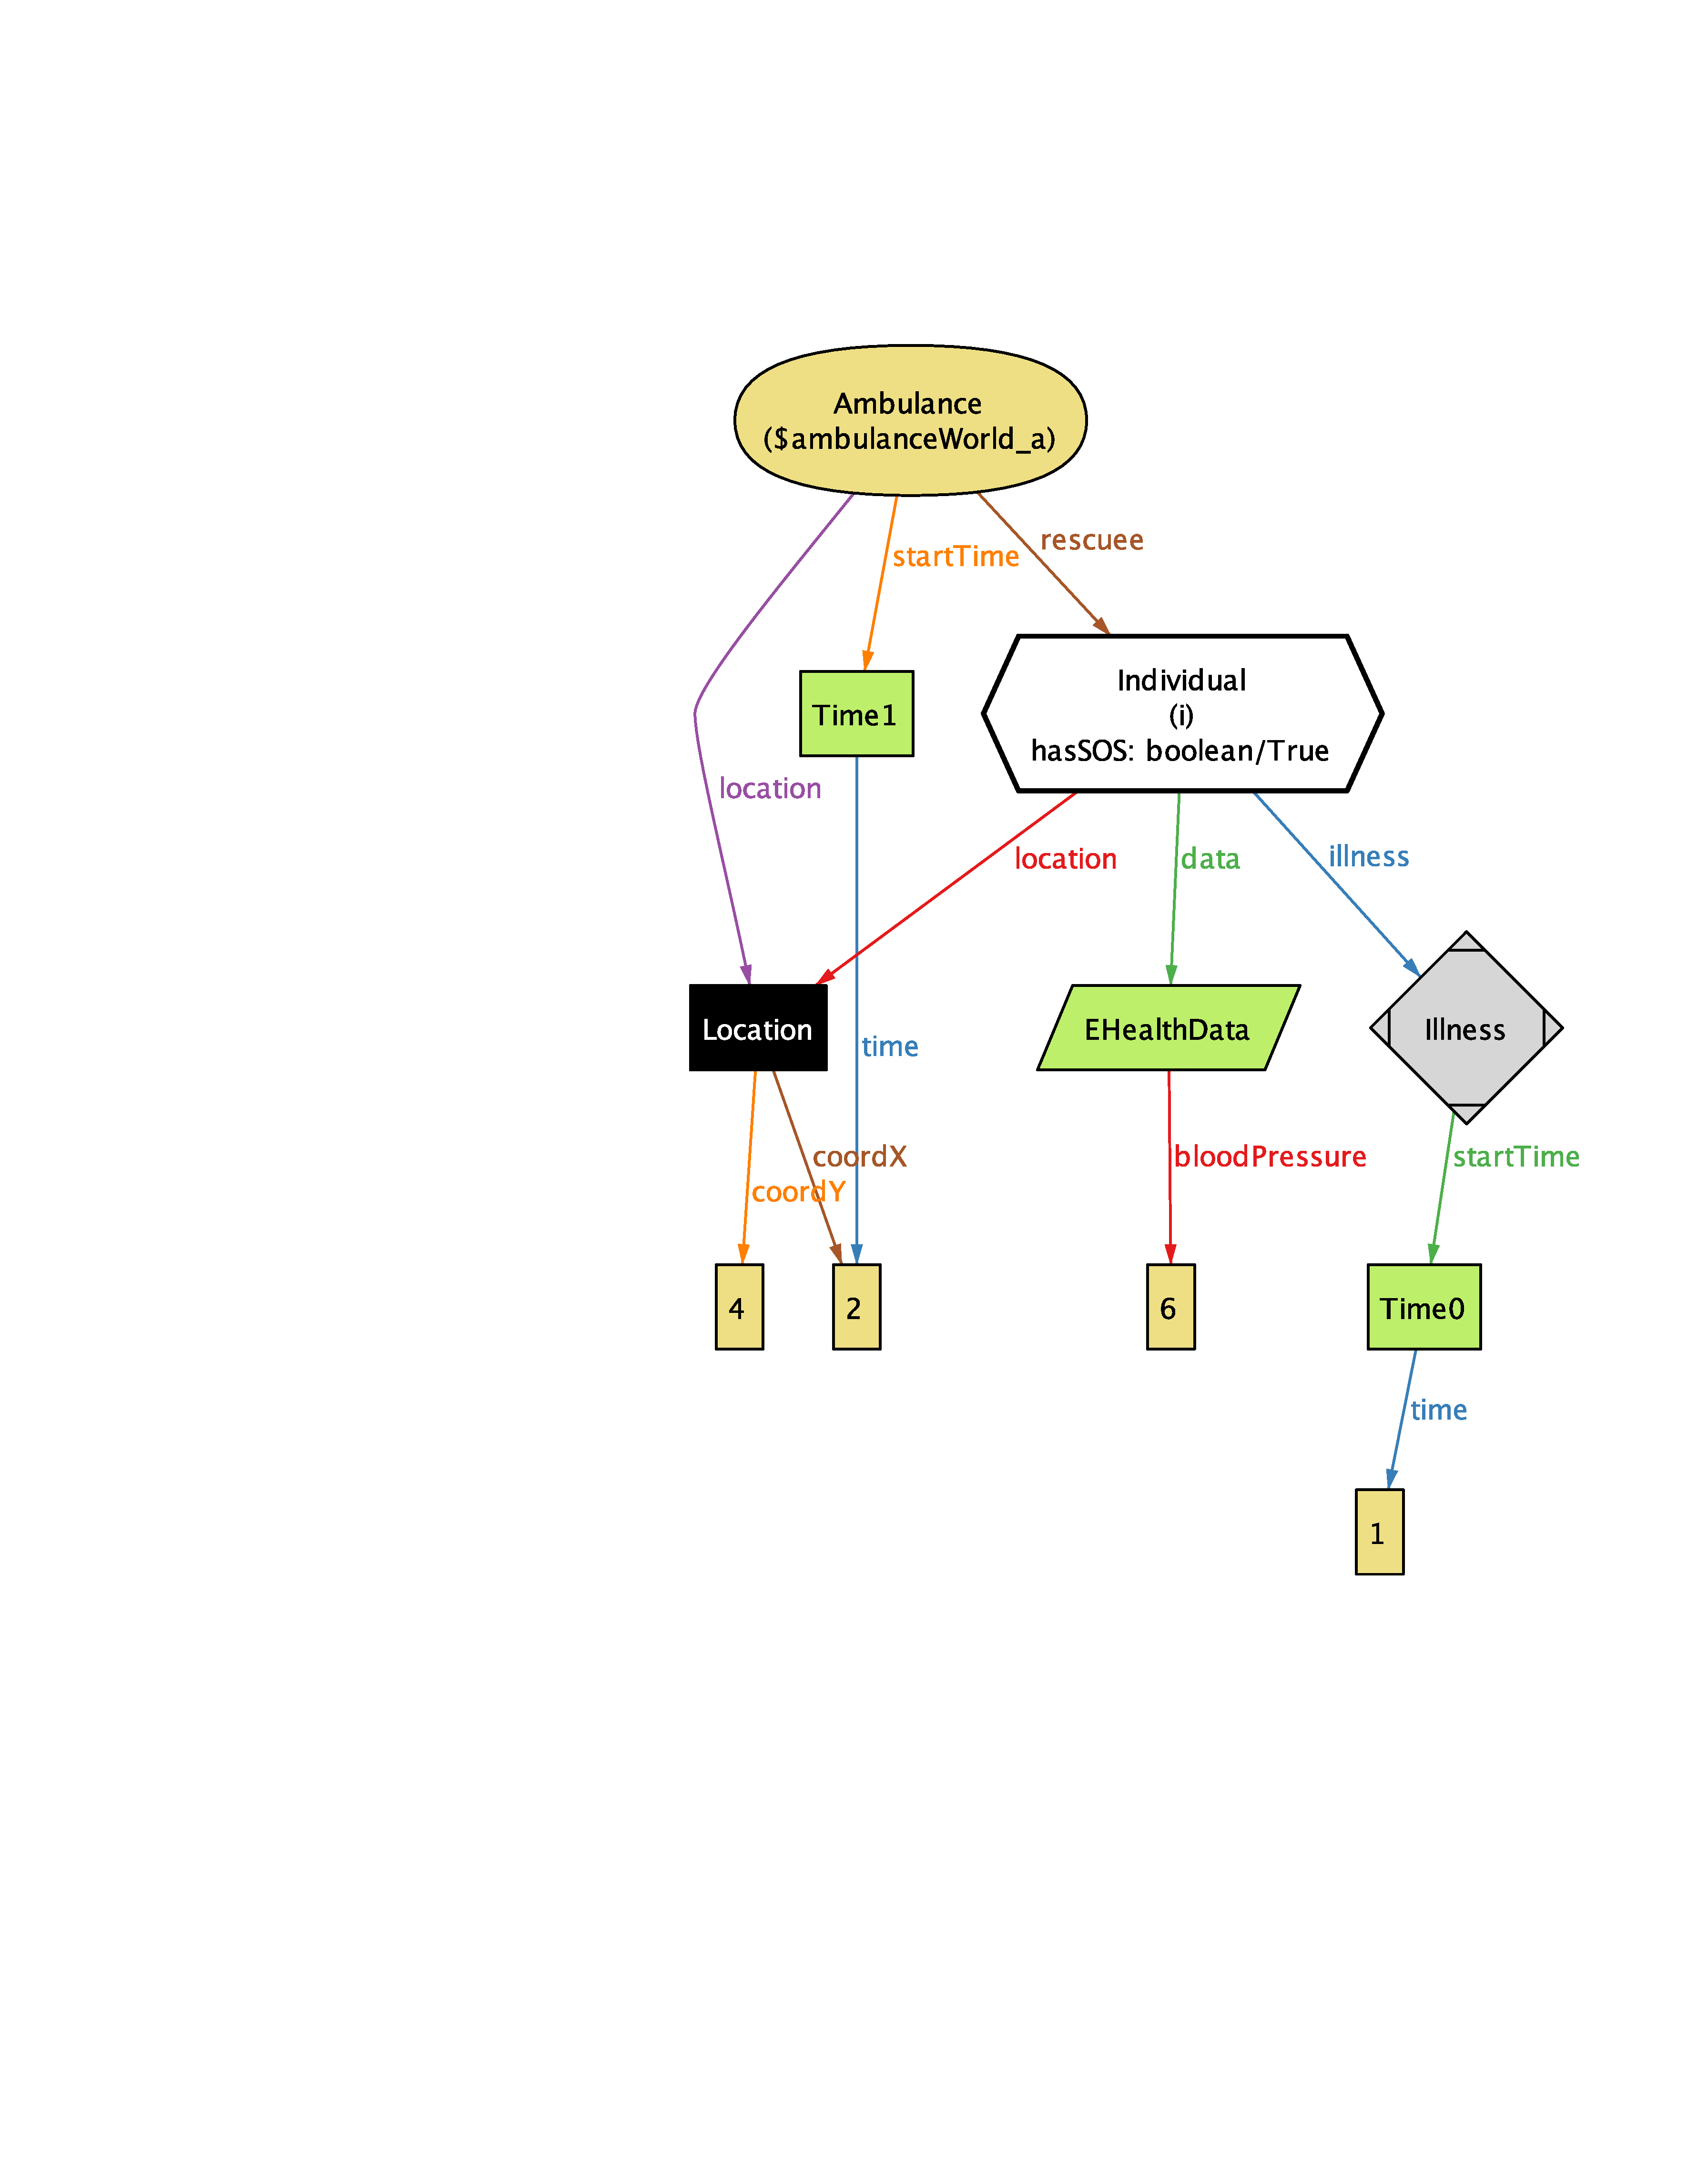
\includegraphics[width=0.9\linewidth]{resources/Alloy/ambulance}}
\caption{World generated by \texttt{ambulanceWorld} predicate}\label{f:ambWorld}
\end{figure}

\subsection{Specific requests}
In Figure \ref{f:specWorld}, it is shown a case in which a third party had sent two distinct specific request but only one is being accepted. 
Note that the third party can effectively monitor only the individual who has accepted the requests.

\begin{lstlisting}[numbers=none]
run specificRequestWorld for 5 but 2 Request, 2 Individual, 1 ThirdParty, 2 EHealthData, 0 EHealthDataGroup, 5 Int
\end{lstlisting}

\begin{figure}[!ht]
\centering
\fbox{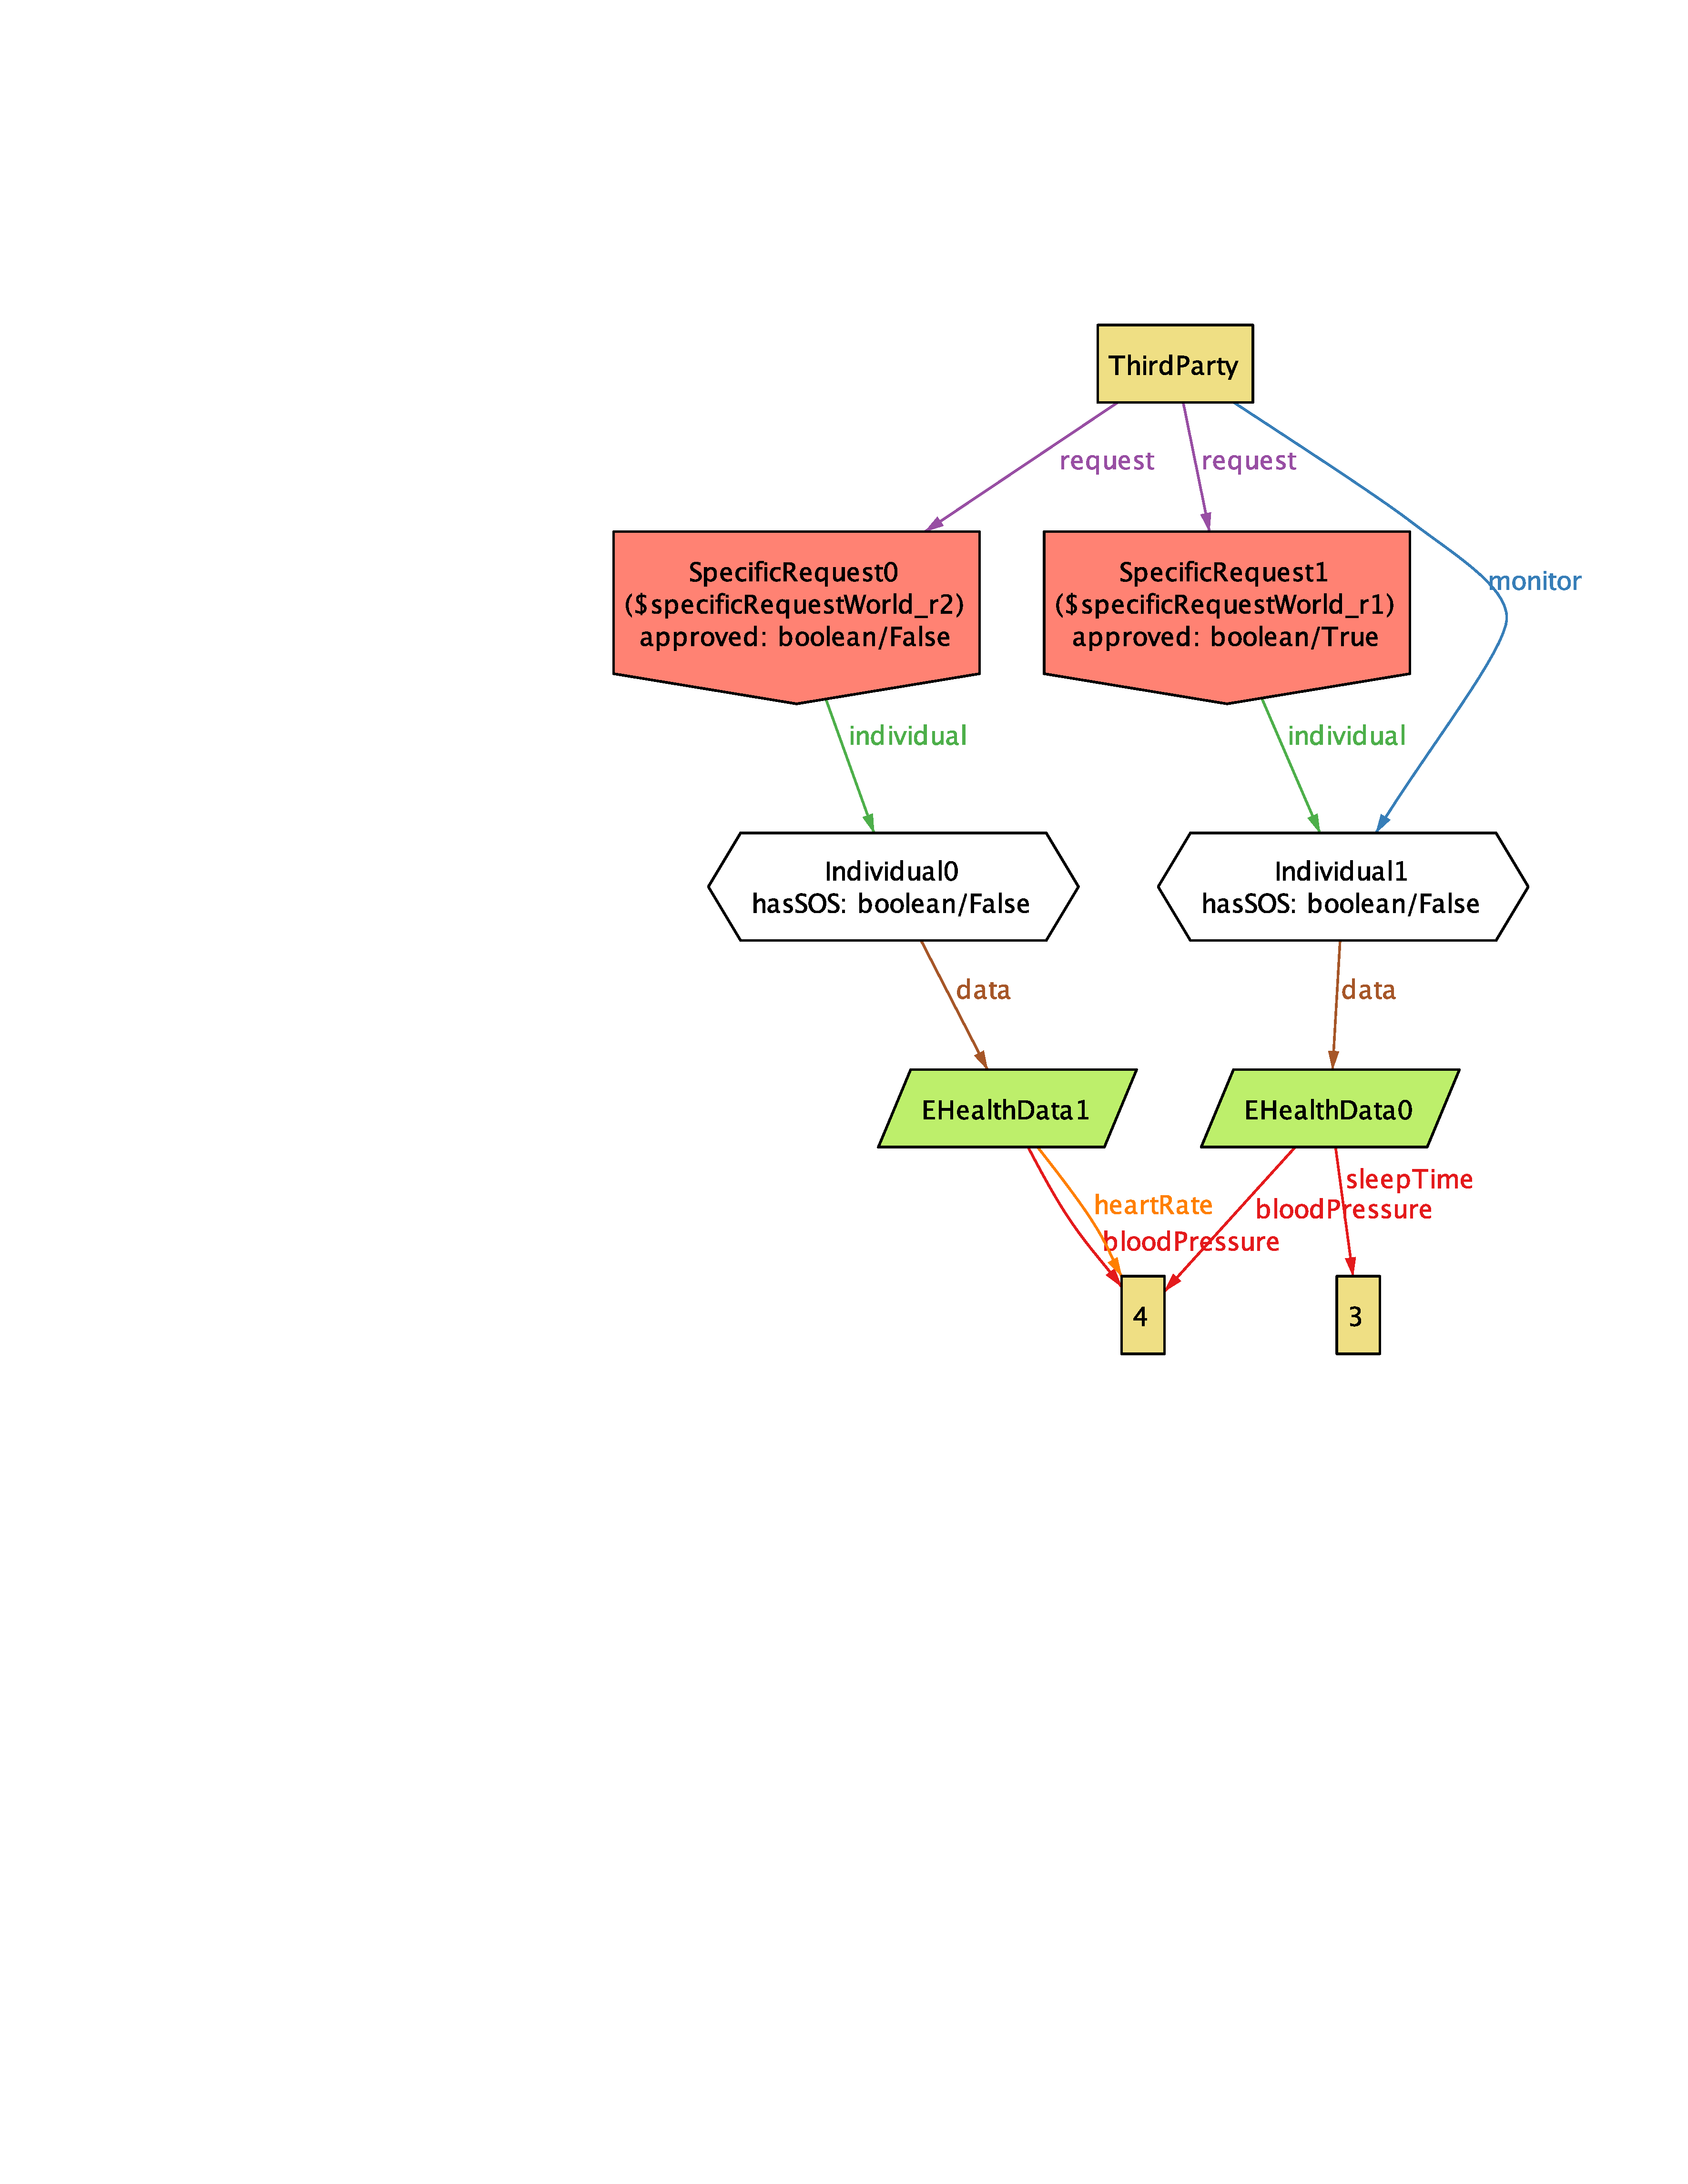
\includegraphics[scale=0.4]{resources/Alloy/specific}}
\caption{World generated by \texttt{specificRequestWorld} predicate}\label{f:specWorld}
\end{figure}


\subsection{Group requests}
Similarly to the previous, Figure \ref{f:groupWorld} shows a third party that had forwarded two group data requests. 
Note that only one respect the privacy constraint and therefore the third party can access only to one group data.
\begin{lstlisting}[numbers=none]
run groupRequestWorld for 6 but 2 Request, 1 ThirdParty, 5 Int
\end{lstlisting}

\begin{figure}[!ht]
\centering
\fbox{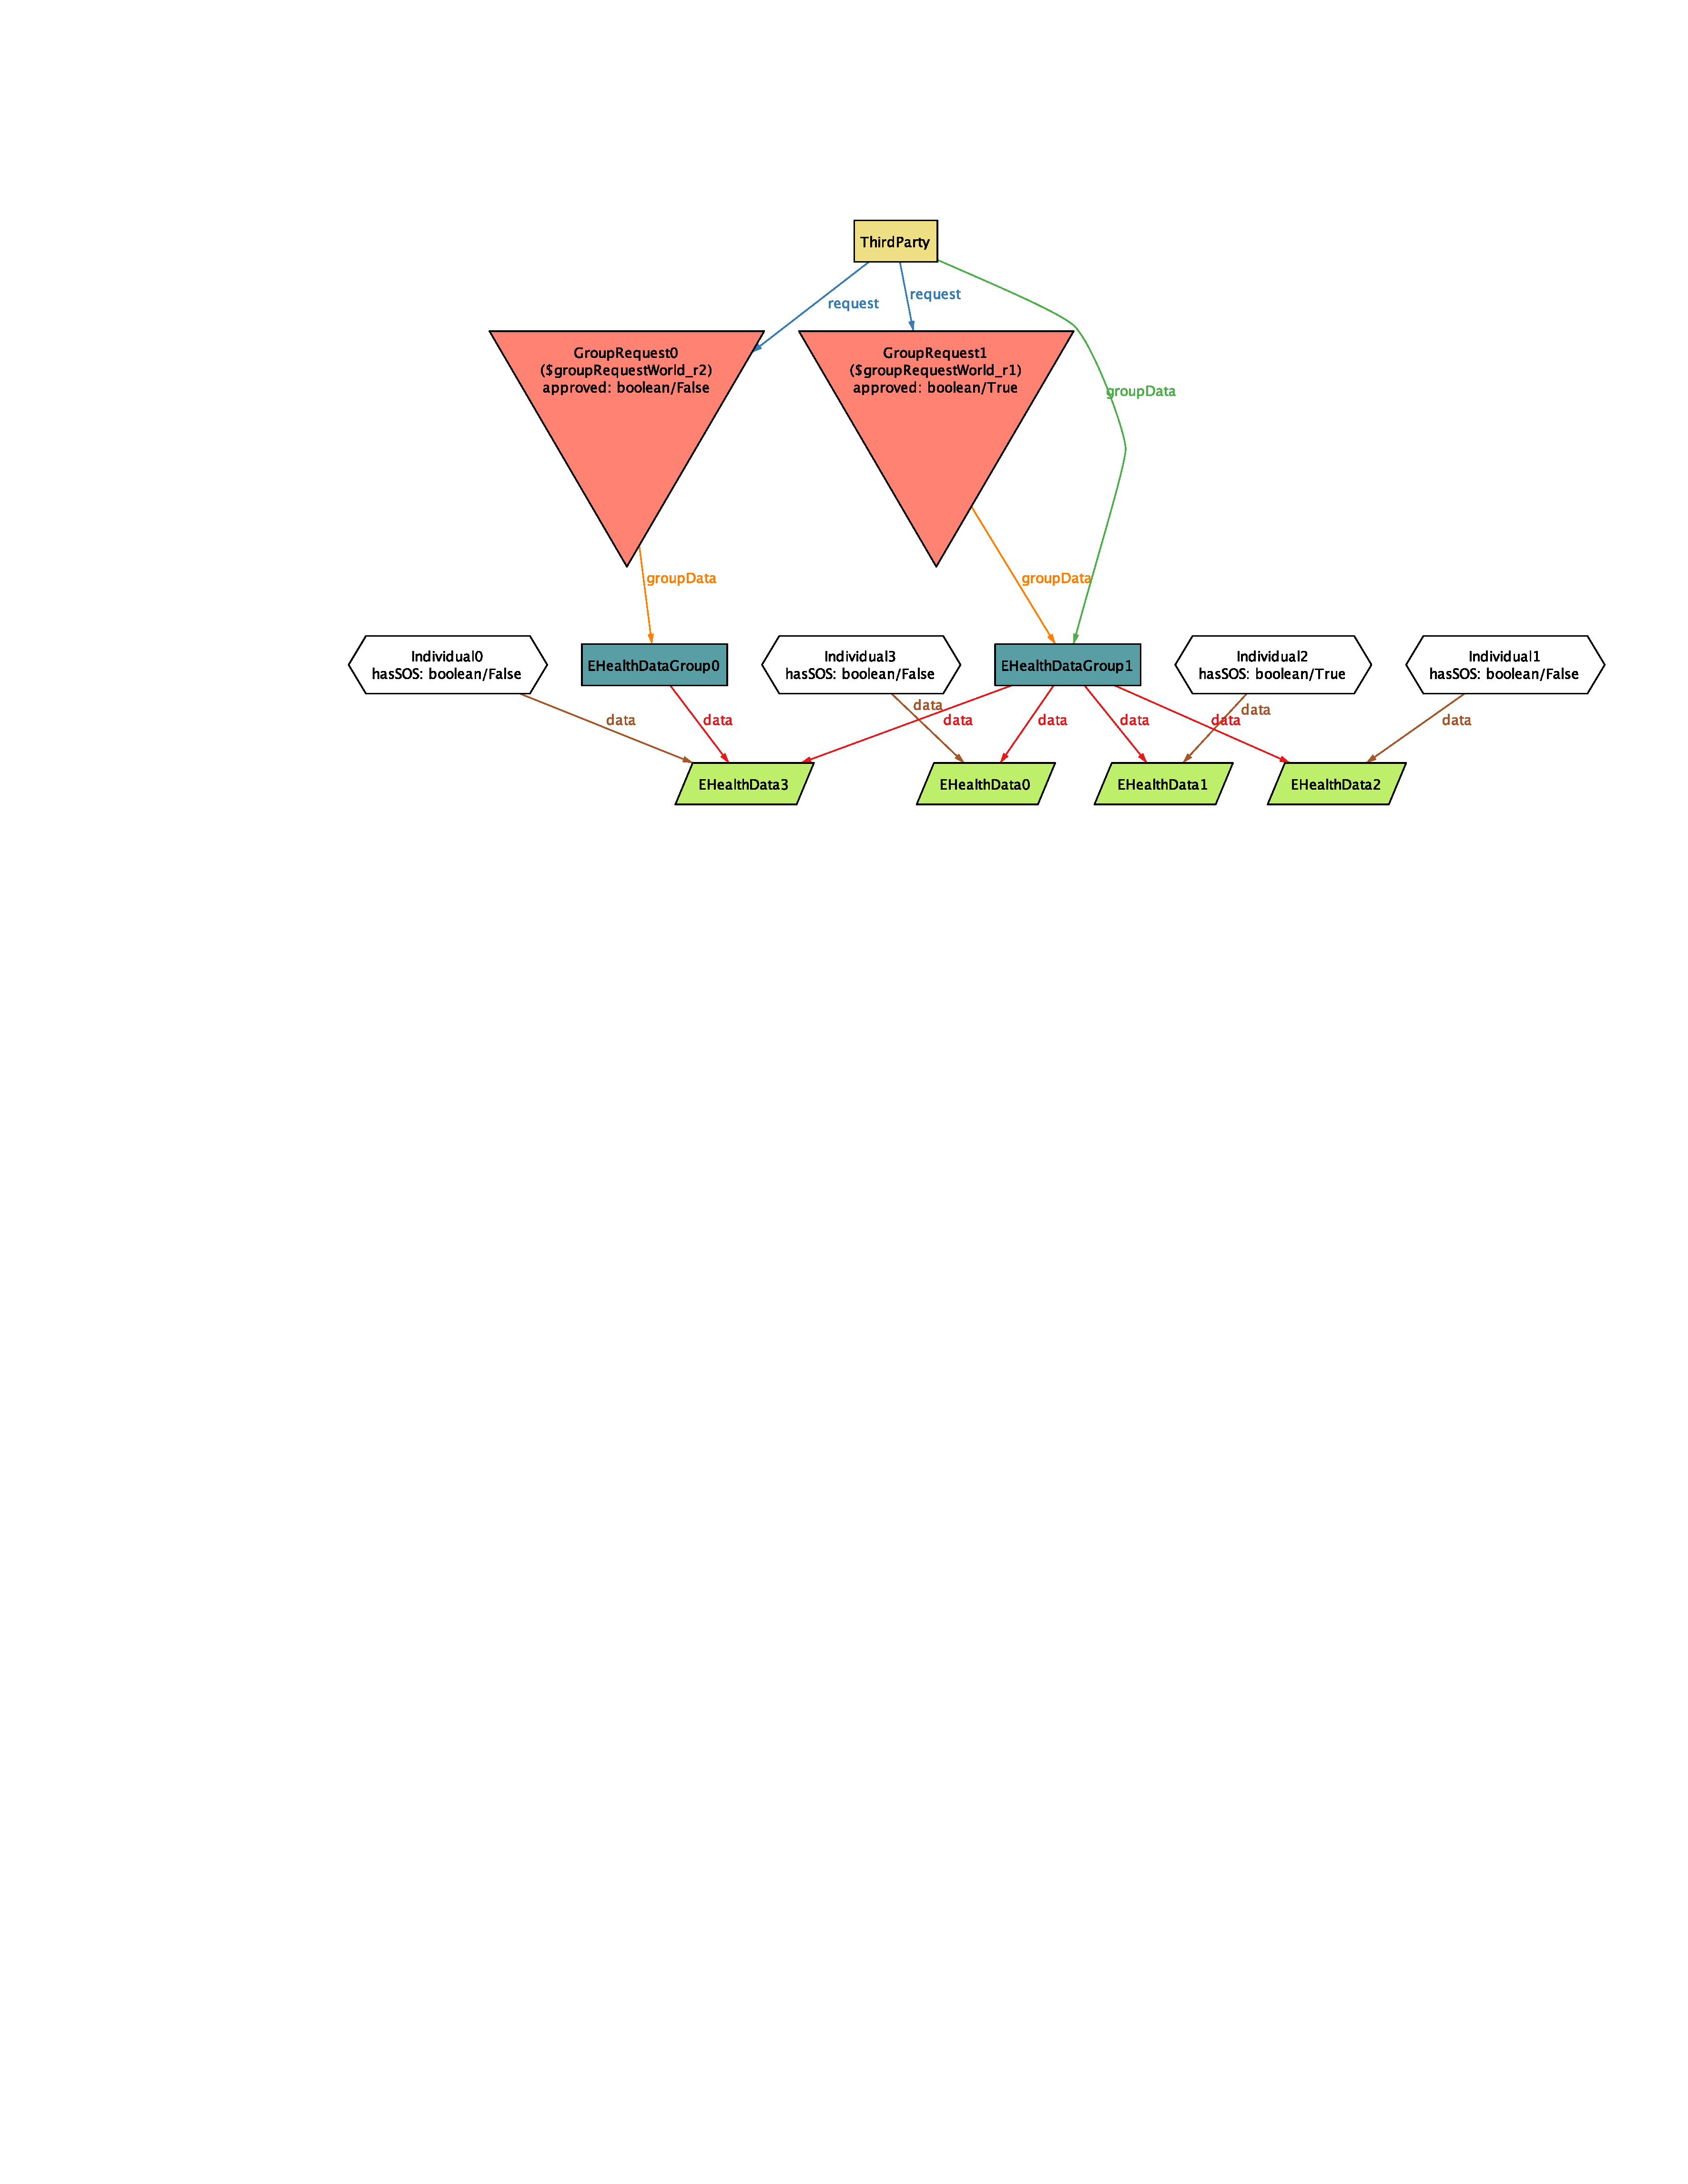
\includegraphics[scale=0.5, angle=-90]{resources/Alloy/group}}
\caption{World generated by \texttt{groupRequestWorld} predicate}\label{f:groupWorld}
\end{figure}

\section{Alloy results}
The checking of the four assertions defined in the model produce the results shown in Figure \ref{f:assertion}


\begin{figure}[!ht]
\centering
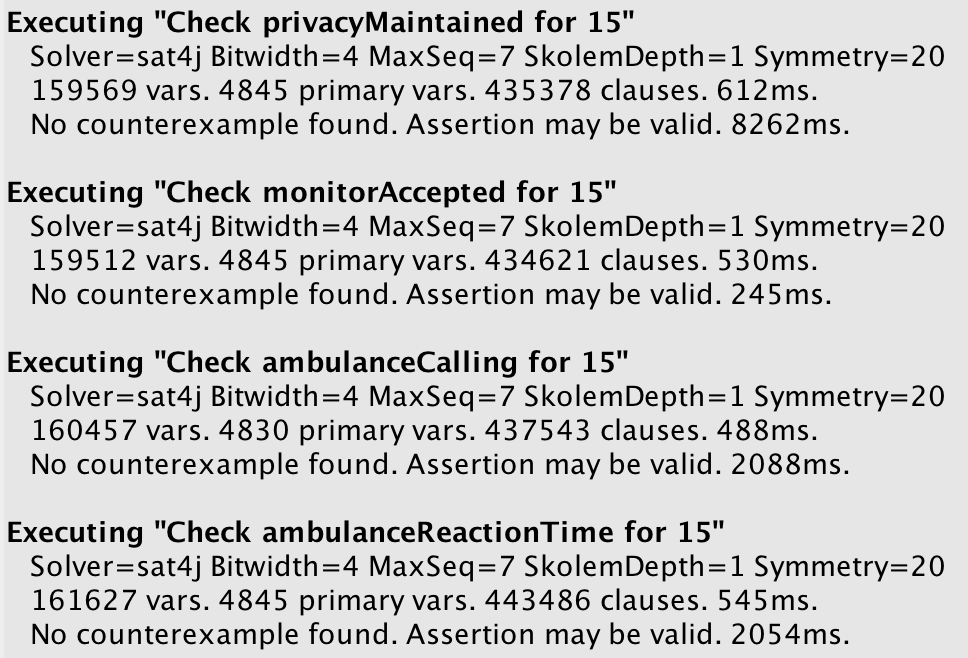
\includegraphics[scale=0.8]{resources/Alloy/assertion}
\caption{Checking of the four assertions}\label{f:assertion}
\end{figure}







